\begin{titlepage}
\newcommand{\HRule}{\rule{\linewidth}{0.5mm}}
\center
\textsc{\LARGE Instituto Tecnológico de Buenos Aires}\\[1.5cm]
\textsc{\Large Electrónica III}\\[0.5cm]

\HRule \\[0.4cm]
{ \huge \bfseries Trabajo Práctico de Laboratorio 1}\\[0.4cm] % Title of your document
\HRule \\[1.5cm]

\begin{minipage}{0.4\textwidth}
\begin{flushleft} \large
\emph{Grupo 4:}\\
Lisandro \textsc{Alvarez} 57771\\
Milton \textsc{Delgado} 56451\\
Paulo \textsc{Navarro} 57775\\
Matías \textsc{Fogg} 56252\\
\end{flushleft}
\end{minipage}
~
\begin{minipage}{0.4\textwidth}
\begin{flushright} \large
\emph{Profesor:} \\
Kevin \textsc{Dewald}\\
\end{flushright}
\end{minipage}\\[4cm]
% If you don't want a supervisor, uncomment the two lines below and remove the section above %\Large \emph{Author:}\\ %John \textsc{Smith}\\[3cm] % Your name

%{\large \today}\\[3cm] % Date, change the \today to a set date if you want to be precise
\begin{minipage}{0.4\textwidth}
\begin{flushleft} \large
Presentado: 5/9/2018\\
Corrección:\\
\end{flushleft}
\end{minipage}
\vfill % Fill the rest of the page with whitespace

\end{titlepage}

%%% Begin document
\begin{document}
\maketitle

% The \input command appends the content of the file directly into the document.
\newpage
\section*{Ejercicio 1}
Los sistemas digitales disponen de registros y buses de tamaños específicos que limitan la cantidad de bits disponibles para la representación de los datos. Es habitual mencionar que el sistema trabaja con datos de 8, 16, 32 bits, o en punto flotante de simple/doble precisión. Por lo tanto, las representaciones que se utilizan tienen limitaciones, y los cálculos están siempre sujetos a aproximaciones y por ende a errores. Para caracterizar los sistemas de representación y compararlos se definen tres parámetros importantes:    
\begin{itemize}
	\item Rango: El rango de un sistema está dado por el número mínimo y el número máximo representables. Por ejemplo, en binario con cinco dígitos es [0, 31]
	\item Capacidad de representación: Es la cantidad de tiras distintas que se pueden representar. Por ejemplo, si tengo un sistema restringido a 5 bits, sería 25 tiras, es decir, 32. 
	\item Resolución: Es la mínima diferencia entre un número representable y el siguiente. Por ejemplo, en binario con dos dígitos fraccionarios es 0.01.  
\end{itemize}
En este ejercicio se implementó un código en C para determinar, a partir de la cantidad de dígitos de la parte entera y fraccionaria de cierta convención de punto fijo (signado y no signado), el rango, la capacidad y la resolución.



\section*{Ejercicio 2}
\subsection*{PARTE 1}

Teniendo la expresi�n en maxit�rminos: $f(d,c,b,a)=\prod (M_{0},M_{1},M_{5},M_{7},M_{8},M_{10},M_{14},M_{15})$
Realizaremos una simplificaci�n de esta productoria con �lgebra booleana,
pero antes identificaremos cada t�rmino:

Maxit�rminos: \\
$M_{0}= d+c+b+a\ ;$ 
$M_{1}= d+c+b+\overline{a}\ ;$ 
$M_{5}=d+\overline{c}+b+\overline{a}\ ;$ 
$M_{7}=d+\overline{c}+\overline{b}+\overline{a}\ ;$ \\
$M_{8}=\overline{d}+c+b+a\ ;$
$M_{10}=\overline{d}+c+\overline{b}+a\ ;$
$M_{14}=\overline{d}+\overline{c}+\overline{b}+a\ ;$
$M_{15}=\overline{d}+\overline{c}+\overline{b}+\overline{a}$ 

Ahora pasaremos a realizar la productoria:

$f(d,c,b,a) = M_{0} * M_{1} * M_{5} * M_{7} * M_{8} * M_{10} * M_{14} * M_{15} \\ 
f=(d+c+b+a)*(d+c+b+\overline{a})*(d+\overline{c}+b+\overline{a})*(d+\overline{c}+\overline{b}+\overline{a})* \\ (\overline{d}+c+b+a)*(\overline{d}+c+\overline{b}+a)*(\overline{d}+\overline{c}+\overline{b}+a)*(\overline{d}+\overline{c}+\overline{b}+\overline{a})$

Podemos notar que entre el maxit�rmino $M_{0}$ y $M_{1}$ se puede
aplicar la propiedad de combinaci�n y eliminar la variable $a$ ya
que:

$(d+c+b+a)*(d+c+b+\overline{a})=(d+c+b)$

De la misma forma en los t�rminos $M_{5}$ y $M_{7}$ se puede eliminar
la variable $b$, entre los t�rminos $M_{8}$ y $M_{10}$ se elimina
la variable $b$, y entre los t�rminos $M_{14}$ y $M_{15}$ se elimina
la variable $a$. Entonces se puede eliminar algunas variables y reducir
la ecuaci�n a:

$f(d,c,b,a) = (d+c+b)*(d+\overline{c}+\overline{a})*(\overline{d}+c+a)*(\overline{d}+\overline{c}+\overline{b})$

Para no complicar tanto la ecuaci�n y no enredarnos vamos a separar
la funci�n principal en 2, para que $f(d,c,b,a)=f_{1}(d,c,b,a)*f_{2}(d,c,b,a)$,
definiendo a cada una de la siguiente forma:

$f_{1}(d,c,b,a)=(d+c+b)*(\overline{d}+\overline{c}+\overline{b})$
y $f_{2}(d,c,b,a)=(\overline{d}+c+a)*(d+\overline{c}+\overline{a})$

A partir de ahora analizaremos solo $f_{1}$ y veremos el resultado
que se obtiene. No haremos el an�lisis para $f_{2}$ ya que ser� el
mismo pero con un resultado final distinto. 

$f_{1}=(d+c+b)*(\overline{d}+\overline{c}+\overline{b})=d*\overline{c}+d*\overline{b}+c*\overline{d}+c*\overline{b}+b*\overline{d}+b*\overline{c}+d*\overline{d}+c*\overline{c}+b*\overline{b}$

Vamos a recordar un teorema de 1 variblae $X*\overline{X}=0$ y a
reordenar los t�rminos:

$f_{1}= b*\overline{c} + \overline{c}*d + \overline{b}*d + b*\overline{d} +  \overline{d}*c + \overline{b}*c $

Para poder seguir reduciendo la ecuaci�n vamos a utilizar la propiedad
del consenso $(x+y)*(y+z)*(\overline{x}+z)=(x+y)*(\overline{x}+z)$
con los primeros 3 t�rminos, y luego con los segundos 3 t�rminos,
entonces:

$b*\overline{c}+\overline{c}*d+\overline{b}*d = b*\overline{c}+\overline{b}*d$ \ ;\  $b*\overline{d}+\overline{d}*c+\overline{b}*c = b*\overline{d} + \overline{b}*c$

$f_{1}=b*\overline{c} + \overline{b}*d + b*\overline{d} + \overline{b}*c=(\ b*(\overline{c}+\overline{d})\ +\ \overline{b}*(c+d)\ )$

De la misma forma, para $f_{2}$ quedar�:

$f_{2}=a*\overline{c} + a*\overline{d} + \overline{a}*c + \overline{a}*d =(\ a*(\overline{c}+\overline{d})\ +\ \overline{a}*(c+d)\ ) $

Volviendo a $f$ obtenemos:

$f=f_{1}*f_{2}=(\ b*(\overline{c}+\overline{d})\ +\ \overline{b}*(c+d)\ )*(\ a*(\overline{c}+\overline{d})\ +\ \overline{a}*(c+d)\ )$

Aplicando la propiedad distributiva:

$f=ab(\overline{c}+d)(\overline{c}+\overline{d})+a\overline{b}(c+d)(\overline{c}+d)+\overline{a}b(c+\overline{d})(\overline{c}+\overline{d})+\overline{a}\overline{b}(c+\overline{d})(c+d)$

Para reducir estos t�rminos utilizamos la propiedad de combinaci�n
de 2 variables, ya que $(X+Y)(X+\overline{Y})=X$:

$(\overline{c}+d)(\overline{c}+\overline{d})=\overline{c} \ ;\ (c+d)(\overline{c}+d)=d\ ;\ (c+\overline{d})(\overline{c}+\overline{d})=\overline{d}\ ;\ (c+\overline{d})(c+d)=c$

Entonces como resultado final obtenemos que:

$f(d,c,b,a)=ab\overline{c}+a\overline{b}d+\overline{a}b\overline{d}+\overline{a}\overline{b}c=\overline{d}b\overline{a}+d\overline{b}a+\overline{c}ba+c\overline{b}\overline{a}$

\subsection*{PARTE 2}

Ahora veremos que suceder�a si vieramos el problema desde los mapas
de Karnaugh, teniendo los mismos maxit�rminos.

\begin{tabular}{|c|c|c|c|c|}
\hline 
dc \textbackslash{} ba & 00 & 01 & 11 & 10\tabularnewline
\hline 
00 & 0 & 1 & 1 & 0\tabularnewline
\hline 
01 & 0 & 0 & 1 & 1\tabularnewline
\hline 
11 & 1 & 0 & 0 & 1\tabularnewline
\hline 
10 & 1 & 1 & 0 & 0\tabularnewline
\hline 
\end{tabular}

Agrupamos todos los maxit�rminos de a pares verticales, $M_{0}$ con
$M_{1}$, $M_{5}$ con $M_{7}$, $M_{8}$ con $M_{10}$ y $M_{14}$
con $M_{15}$. Al primer par lo llamaremos $I_{1}$, al segundo $I_{2}$,
al tercero $I_{3}$ y el �ltimo lo llamaremos $I_{4}$

\subsection*{3 PARTE}

\selectlanguage{friulan}%
DaDo el resultado final, el circuito utilizando solo compuertas NOT,
AND y OR es el siguiente:

\begin{figure}
\caption{\foreignlanguage{english}{TP1EJ2c\_electroiii}}

\selectlanguage{english}%
\selectlanguage{friulan}%
\end{figure}

\selectlanguage{english}%

\subsection*{4 PARTE}

\selectlanguage{spanish}%
Para utilizar solo compuertas NAND por ser el grupo 4, necesitamos
trabajar sobre $f(d,c,b,a)$ viendo que si se niega 2 veces la ecuaci�n
final para mantener la igualdad, luego de aplicar el teorema de De
Morgan, obtendremos un resultado que puede tratarse de un conjunto
de compuertas NAND y NOT:

$\overline{\overline{f}}=\overline{\overline{\overline{d}b\overline{a}+d\overline{b}a+\overline{c}ba+c\overline{b}\overline{a}}}=\overline{\overline{(\overline{d}b\overline{a})} * \overline{(d\overline{b}a)} * \overline{(\overline{c}ba)} * \overline{(c\overline{b}\overline{a})}}$

Analizando el nuevo resultado final podemos notar que se trata solo
de productos negados y algunas entradas negadas, siendo as� necesarias
5 compuertas NAND's y 4 NOT's, o simplemente 9 NAND's (el ejercicio
solo pide NAND). El circuito ser�a el siguiente:

\begin{figure}
\selectlanguage{english}%

\selectlanguage{spanish}%
\caption{TP1EJ2d\_electroiii}

\selectlanguage{english}%
\selectlanguage{spanish}%
\end{figure}

\input{ejercicio3/ejercicio3.tex}
\documentclass[english]{article}

\usepackage{graphicx}
\usepackage{babel}

\begin{document}
\section{Ejercicio 4}
En primer lugar a continuacion se presenta la tabla de verdad para la salida, la cual se presenta de la forma Y3, Y2, Y1, Y0 (bit mas significativo al menos significativo y analogamente para la entrada).
\begin{table}[htb] 
\centering  
\begin{tabular}{|c|c|c|c|}  
\hline  
\multicolumn{4}{|c|}{\textbf{Entradas}} \\ \hline  
\textbf{A3} & \textbf{A2} & \textbf{A1} & \textbf{A0} \\ \hline  
\textbf{0} & \textbf{0} & \textbf{0} & \textbf{0} \\ \hline  
\textbf{0} & \textbf{0} & \textbf{0} & \textbf{1} \\ \hline  
\textbf{0} & \textbf{0} & \textbf{1} & \textbf{0} \\ \hline  
\textbf{0} & \textbf{0} & \textbf{1} & \textbf{1} \\ \hline  
\textbf{0} & \textbf{1} & \textbf{0} & \textbf{0} \\ \hline  
\textbf{0} & \textbf{1} & \textbf{0} & \textbf{1} \\ \hline  
\textbf{0} & \textbf{1} & \textbf{1} & \textbf{0} \\ \hline  
\textbf{0} & \textbf{1} & \textbf{1} & \textbf{1} \\ \hline  
\textbf{1} & \textbf{0} & \textbf{0} & \textbf{0} \\ \hline  
\textbf{1} & \textbf{0} & \textbf{0} & \textbf{1} \\ \hline  
\textbf{1} & \textbf{0} & \textbf{1} & \textbf{0} \\ \hline  
\textbf{1} & \textbf{0} & \textbf{1} & \textbf{1} \\ \hline  
\textbf{1} & \textbf{1} & \textbf{0} & \textbf{0} \\ \hline  
\textbf{1} & \textbf{1} & \textbf{0} & \textbf{1} \\ \hline  
\textbf{1} & \textbf{1} & \textbf{1} & \textbf{0} \\ \hline  
\textbf{1} & \textbf{1} & \textbf{1} & \textbf{1} \\ \hline  
\end{tabular}  
\begin{tabular}{|c|c|c|c|} \hline 
\multicolumn{4}{|c|}{\textbf{Salidas}}                \\ \hline  
\textbf{Y3} & \textbf{Y2} & \textbf{Y1} & \textbf{Y0} \\ \hline  
\textbf{0}  & \textbf{0}  & \textbf{0}  & \textbf{0}  \\ \hline  
\textbf{1}  & \textbf{1}  & \textbf{1}  & \textbf{1}  \\ \hline  
\textbf{1}  & \textbf{1}  & \textbf{1}  & \textbf{0}  \\ \hline  
\textbf{1}  & \textbf{1}  & \textbf{0}  & \textbf{1}  \\ \hline  
\textbf{1}  & \textbf{1}  & \textbf{0}  & \textbf{0}  \\ \hline  
\textbf{1}  & \textbf{0}  & \textbf{1}  & \textbf{1}  \\ \hline  
\textbf{1}  & \textbf{0}  & \textbf{1}  & \textbf{0}  \\ \hline  
\textbf{1}  & \textbf{0}  & \textbf{0}  & \textbf{1}  \\ \hline  
\textbf{1}  & \textbf{0}  & \textbf{0}  & \textbf{0}  \\ \hline  
\textbf{0}  & \textbf{1}  & \textbf{1}  & \textbf{1}  \\ \hline  
\textbf{0}  & \textbf{1}  & \textbf{1}  & \textbf{0}  \\ \hline  
\textbf{0}  & \textbf{1}  & \textbf{0}  & \textbf{1}  \\ \hline  
\textbf{0}  & \textbf{1}  & \textbf{0}  & \textbf{0}  \\ \hline  
\textbf{0}  & \textbf{0}  & \textbf{1}  & \textbf{1}  \\ \hline  
\textbf{0}  & \textbf{0}  & \textbf{1}  & \textbf{0}  \\ \hline  
\textbf{0}  & \textbf{0}  & \textbf{0}  & \textbf{1}  \\ \hline  
\end{tabular} 
\end{table}

Lo siguiente que se realizo fueron los mapas de Karnaugh para cada bit de la salida, para Y0 arriba a la izquierda,para Y1 arriba a la derecha, para Y2 abajo ala izquierda y para Y3 abajo a la derecha:
\begin{table}[htb] 
\centering
\begin{tabular}{|c|c|c|c|l|}
\hline
\textbf{A3A2} & \textbf{00} & \textbf{01} & \textbf{11} & \textbf{10} \\ \hline
\textbf{A1A0} & \multicolumn{4}{c|}{\textbf{}}                        \\ \hline
\textbf{00}   & \textbf{0}  & \textbf{0}  & \textbf{0}  & \textbf{0}  \\ \hline
\textbf{01}   & \textbf{1}  & \textbf{1}  & \textbf{1}  & \textbf{1}  \\ \hline
\textbf{11}   & \textbf{1}  & \textbf{1}  & \textbf{1}  & \textbf{1}  \\ \hline
\textbf{10}   & \textbf{0}  & \textbf{0}  & \textbf{0}  & \textbf{0}  \\ \hline
\end{tabular}
\begin{tabular}{|c|c|c|c|l|}
\hline
\textbf{A3A2} & \textbf{00} & \textbf{01} & \textbf{11} & \textbf{10} \\ \hline
\textbf{A1A0} & \multicolumn{4}{c|}{\textbf{}}                        \\ \hline
\textbf{00}   & \textbf{0}  & \textbf{0}  & \textbf{0}  & \textbf{0}  \\ \hline
\textbf{01}   & \textbf{1}  & \textbf{1}  & \textbf{1}  & \textbf{1}  \\ \hline
\textbf{11}   & \textbf{0}  & \textbf{0}  & \textbf{0}  & \textbf{0}  \\ \hline
\textbf{10}   & \textbf{1}  & \textbf{1}  & \textbf{1}  & \textbf{1}  \\ \hline
\end{tabular}
\begin{tabular}{|c|c|c|c|l|}
\hline
\textbf{A3A2} & \textbf{00} & \textbf{01} & \textbf{11} & \textbf{10} \\ \hline
\textbf{A1A0} & \multicolumn{4}{c|}{\textbf{}}                        \\ \hline
\textbf{00}   & \textbf{0}  & \textbf{1}  & \textbf{1}  & \textbf{0}  \\ \hline
\textbf{01}   & \textbf{1}  & \textbf{0}  & \textbf{0}  & \textbf{1}  \\ \hline
\textbf{11}   & \textbf{1}  & \textbf{0}  & \textbf{0}  & \textbf{1}  \\ \hline
\textbf{10}   & \textbf{1}  & \textbf{0}  & \textbf{0}  & \textbf{1}  \\ \hline
\end{tabular}
\begin{tabular}{|c|c|c|c|l|}
\hline
\textbf{A3A2} & \textbf{00} & \textbf{01} & \textbf{11} & \textbf{10} \\ \hline
\textbf{A1A0} & \multicolumn{4}{c|}{\textbf{}}                        \\ \hline
\textbf{00}   & \textbf{0}  & \textbf{1}  & \textbf{0}  & \textbf{1}  \\ \hline
\textbf{01}   & \textbf{1}  & \textbf{1}  & \textbf{0}  & \textbf{0}  \\ \hline
\textbf{11}   & \textbf{1}  & \textbf{1}  & \textbf{0}  & \textbf{0}  \\ \hline
\textbf{10}   & \textbf{1}  & \textbf{1}  & \textbf{0}  & \textbf{0}  \\ \hline
\end{tabular}
\end{table}

Con estos mapas de Karnaugh obtenemos para cada salida las siguientes expresiones en funcion de los minterminos: \\
$Y0 = m_1 . m_3 . m_5 . m_7 m_{13} . m_{15} . m_9 . m_{11}$ \\
$Y1 = m_1 . m_5 . m_{13} . m_9 + m_2 . m_6 . m_{16} . m_{10}$ \\
$Y2 = m_4 . m_{12} + m_1 . m_3 . m_9 . m_{11} + m_3 . m_2 . m_{11} . m_{10}$\\
$Y3 = m_8 + m_4 . m_5 . m_7 . m_6 + m_1 . m_3 . m_5 . m_7 + m_3 . m_2 . m_7 . m_6$\\
Y si procedemos a simplificar obtenemos:
$Y0 = A0$\\
$Y1 = A0 . \overline{A1} + \overline{A0} . A1$\\
$Y2 = A0 . \overline{A2} + A1 . \overline{A2} + \overline{A0} . \overline{A1} . A2$\\
$Y3 = A0 . \overline{A3} + A1 . \overline{A3} + A2 . \overline{A3} + \overline{A0} . \overline{A1} . \overline{A2} . A3$\\
Y por ultimo podemos representar las salidas en funcion de las entradas con las compuertas logicas como se puede observar en los graficos que mostramos a continuacion, donde no representamos Y0 ya que es directamente igual a la entrada A0:

\begin{figure}[htb] 
  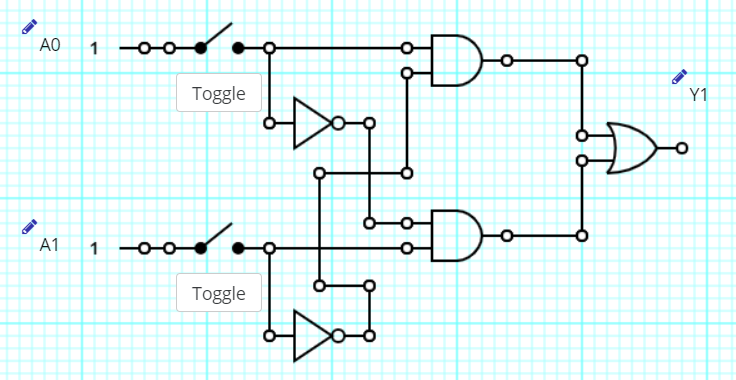
\includegraphics[width=\linewidth]{Y1CompuertasLogicas.png}
\end{figure}

\begin{figure}[htb] 
  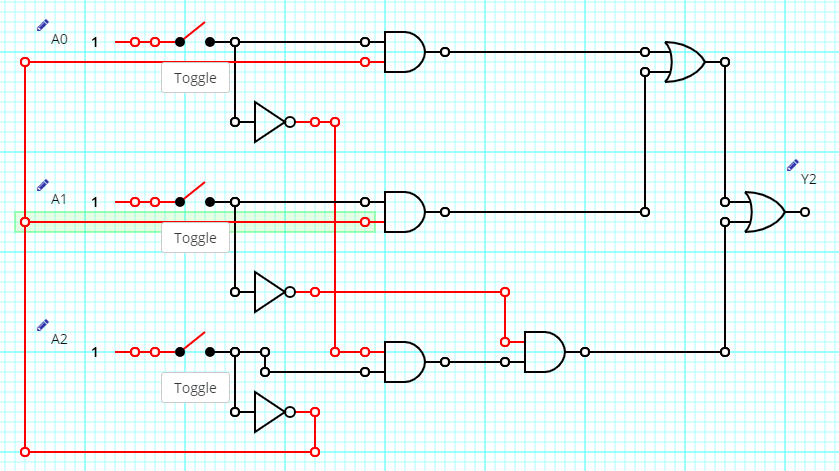
\includegraphics[width=\linewidth]{Y2CompuertasLogicas.png}
\end{figure}

\begin{figure}[htb] 
  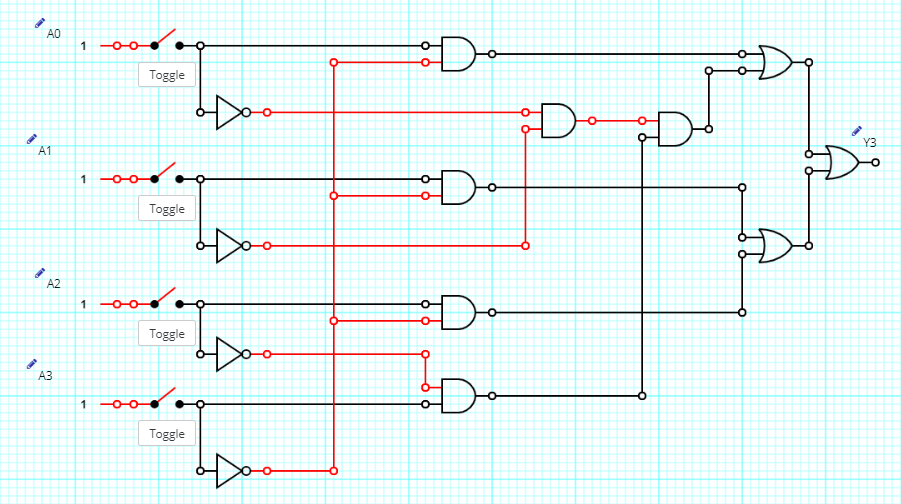
\includegraphics[width=\linewidth]{Y3CompuertasLogicas.png}
\end{figure}

\end{document}

\input{ejercicio5/ejercicio5.tex}
\input{ejercicio6/ejercicio6.tex}


%%% End document
\end{document}
